\documentclass{article}
\usepackage{svg}
\usepackage{amsmath}
\usepackage{amsfonts}
\usepackage{longtable}
\usepackage{booktabs}
\usepackage{hyperref}
\usepackage{mdframed}
\providecommand{\tightlist}{%
  \setlength{\itemsep}{0pt}\setlength{\parskip}{0pt}}
\usepackage{color}
\usepackage{fancyvrb}
\newcommand{\VerbBar}{|}
\newcommand{\VERB}{\Verb[commandchars=\\\{\}]}
\DefineVerbatimEnvironment{Highlighting}{Verbatim}{commandchars=\\\{\}}
% Add ',fontsize=\small' for more characters per line
\usepackage{framed}
\definecolor{shadecolor}{RGB}{248,248,248}
\newenvironment{Shaded}{\begin{snugshade}}{\end{snugshade}}
\newcommand{\KeywordTok}[1]{\textcolor[rgb]{0.13,0.29,0.53}{\textbf{#1}}}
\newcommand{\DataTypeTok}[1]{\textcolor[rgb]{0.13,0.29,0.53}{#1}}
\newcommand{\DecValTok}[1]{\textcolor[rgb]{0.00,0.00,0.81}{#1}}
\newcommand{\BaseNTok}[1]{\textcolor[rgb]{0.00,0.00,0.81}{#1}}
\newcommand{\FloatTok}[1]{\textcolor[rgb]{0.00,0.00,0.81}{#1}}
\newcommand{\ConstantTok}[1]{\textcolor[rgb]{0.00,0.00,0.00}{#1}}
\newcommand{\CharTok}[1]{\textcolor[rgb]{0.31,0.60,0.02}{#1}}
\newcommand{\SpecialCharTok}[1]{\textcolor[rgb]{0.00,0.00,0.00}{#1}}
\newcommand{\StringTok}[1]{\textcolor[rgb]{0.31,0.60,0.02}{#1}}
\newcommand{\VerbatimStringTok}[1]{\textcolor[rgb]{0.31,0.60,0.02}{#1}}
\newcommand{\SpecialStringTok}[1]{\textcolor[rgb]{0.31,0.60,0.02}{#1}}
\newcommand{\ImportTok}[1]{#1}
\newcommand{\CommentTok}[1]{\textcolor[rgb]{0.56,0.35,0.01}{\textit{#1}}}
\newcommand{\DocumentationTok}[1]{\textcolor[rgb]{0.56,0.35,0.01}{\textbf{\textit{#1}}}}
\newcommand{\AnnotationTok}[1]{\textcolor[rgb]{0.56,0.35,0.01}{\textbf{\textit{#1}}}}
\newcommand{\CommentVarTok}[1]{\textcolor[rgb]{0.56,0.35,0.01}{\textbf{\textit{#1}}}}
\newcommand{\OtherTok}[1]{\textcolor[rgb]{0.56,0.35,0.01}{#1}}
\newcommand{\FunctionTok}[1]{\textcolor[rgb]{0.00,0.00,0.00}{#1}}
\newcommand{\VariableTok}[1]{\textcolor[rgb]{0.00,0.00,0.00}{#1}}
\newcommand{\ControlFlowTok}[1]{\textcolor[rgb]{0.13,0.29,0.53}{\textbf{#1}}}
\newcommand{\OperatorTok}[1]{\textcolor[rgb]{0.81,0.36,0.00}{\textbf{#1}}}
\newcommand{\BuiltInTok}[1]{#1}
\newcommand{\ExtensionTok}[1]{#1}
\newcommand{\PreprocessorTok}[1]{\textcolor[rgb]{0.56,0.35,0.01}{\textit{#1}}}
\newcommand{\AttributeTok}[1]{\textcolor[rgb]{0.77,0.63,0.00}{#1}}
\newcommand{\RegionMarkerTok}[1]{#1}
\newcommand{\InformationTok}[1]{\textcolor[rgb]{0.56,0.35,0.01}{\textbf{\textit{#1}}}}
\newcommand{\WarningTok}[1]{\textcolor[rgb]{0.56,0.35,0.01}{\textbf{\textit{#1}}}}
\newcommand{\AlertTok}[1]{\textcolor[rgb]{0.94,0.16,0.16}{#1}}
\newcommand{\ErrorTok}[1]{\textcolor[rgb]{0.64,0.00,0.00}{\textbf{#1}}}
\newcommand{\NormalTok}[1]{#1}

\title{Teoría de la Información\\Ejercicios de Entropía y Fuentes de Información}
\date{Curso 2023 - 2024}
\author{Lucas Goiriz Beltrán\\ Instituto de Biología Integrativa de Sistemas\\(I$_2$SysBio; UV-CSIC)\\Departamento de Matemática Aplicada\\Universitat Politècnica de València (UPV)}

\begin{document}
\maketitle

\textbf{
1. Sea $X$ una variable aleatoria que toma valores sobre un alfabeto $\mathcal{A} = \left\{x_1,x_2,x_3,x_4,x_5\right\}$ con las correspondientes probabilidades $P = \left\{0.1,0.2,0.3,0.05,0.35\right\}$. Calcula la entropía de $X$ y compárala con la de una variable aleatoria que tome valores sobre el mismo alfabeto, pero con una distribución uniforme.
}

\vspace{1cm}

\textbf{
2. Sean dos variables aleatorias $X$ e $Y$ que toman valores sobre el alfabeto $\mathcal{A} = \left\{a_1,a_2,a_3,a_4\right\}$ con una distribución de probabilidad conjunta dada por:
}

\begin{table}[htbp!]
\centering
\begin{tabular}{|c|c|c|c|c|}
    \hline
    $Y \ X$ & $1$ & $2$ & $3$ & $4$ \\
    \hline
    1 & $\frac{1}{8}$ & $\frac{1}{16}$ & $\frac{1}{32}$ & $\frac{1}{32}$ \\
    2 & $\frac{1}{16}$ & $\frac{1}{8}$ & $\frac{1}{32}$ & $\frac{1}{32}$ \\
    3 & $\frac{1}{16}$ & $\frac{1}{16}$ & $\frac{1}{16}$ & $\frac{1}{16}$ \\
    4 & $\frac{1}{4}$ & $0$ & $0$ & $0$ \\
    \hline
\end{tabular}
\end{table}


\textbf{
Además se definen las siguientes probabilidades para cada variable aleatoria: $P(X) = \left\{\frac{1}{2},\frac{1}{4},\frac{1}{8},\frac{1}{8}\right\}$ y $P(Y) = \left\{\frac{1}{4},\frac{1}{4},\frac{1}{4},\frac{1}{4}\right\}$. Calcula la entropía de $X$, la entropía de $Y$, la entropía conjunta $H(X,Y)$, la entropía condicional $H(X|Y)$ y la información mutua $I(X;Y)$.
}

\vspace{1cm}

\textbf{
3. Supon que se lanza un dado equilibrado de forma que, si se obtiene 1,2,3 o 4, se lanza una moneda equilibrada una vez y si se obtiene 5 o 6, se lanza la moneda dos veces. ¿Qué cantidad de información se obtiene acerca del número que ha salido en el dado a partir del resultado del número de ``\textit{caras}'' obtenidos en los lanzamientos de moneda?
}

\vspace{1cm}

\textbf{
4. Se define una fuente de información de memoria nula mediante la siguiente tabla:
}

\begin{table}[htbp!]
\centering
\begin{tabular}{|c|c|c|c|c|c|c|c|c|}
    \hline
    $s_i$ & $s_1$ & $s_2$ & $s_3$ & $s_4$ & $s_5$ & $s_6$ & $s_7$ & $s_8$\\
    \hline
    $P(s_i)$ & $0.3$ & $0.21$ & $0.17$ & $0.13$ & $0.09$ & $0.07$ & $0.01$ & $0.02$ \\
    \hline
\end{tabular}
\end{table}

\textbf{
    \begin{itemize}
        \item Calcula la entropía de la fuente.
        \item ¿Cómo cambia la entropía en el caso de símbolos equiprobables?
    \end{itemize}
}

\vspace{1cm}

\textbf{
5. Sea una fuente de información de memoria nula con el alfabeto $\mathcal{A}=\left\{a_1,a_2,a_3,a_4,a_5,a_6\right\}$ y probabilidad $p\left(a_i\right) = ip\left(a_1\right)$ para $i=1,2,3,4,5,6$. Calcula la entropía de la fuente.
}

\vspace{1cm}

\textbf{
6. Considera una fuente binaria de memoria nula.
\begin{itemize}
    \item Calcula la entropía de la fuente si la probabilidad de uno de los símbolos es $p$.
    \item Calcula las entropías para la segunda y tercera extensión de la fuente.
\end{itemize} 
}

\vspace{1cm}

\textbf{
7. Sea $\mathcal{S}=\left(\mathcal{A},P\right)$ una fuente de información de memoria nula en la que $\mathcal{A} = \left\{a,b,c,d\right\}$ y sometida a la restrucción $p(a)=0.4$. Calcule las posibles probabilidades de los símbolos $b$, $c$ y $d$ de forma que la entropía de la fuente sea:
}
\begin{itemize}
    \item \textbf{Máxima.}
    \item \textbf{Mínima.}
\end{itemize}
\textbf{
Muestra el valor de la entropía en ambos casos.
}

\pagebreak

\textbf{
8. Suponga una fuente de información que emite como símbolos el número de caras que se obtienen al lanzar dos veces una moneda equilibrada. Calcule la entropía de la fuente de información y de la fuente de información extendida de orden 2.
}

\vspace{1cm}

\textbf{
9. Se define una fuente de Markov de segundo orden sobre el alfabeto binario definida mediante el siguiente diagrama de estados:
}

\begin{figure}[htbp!]
    \centering
    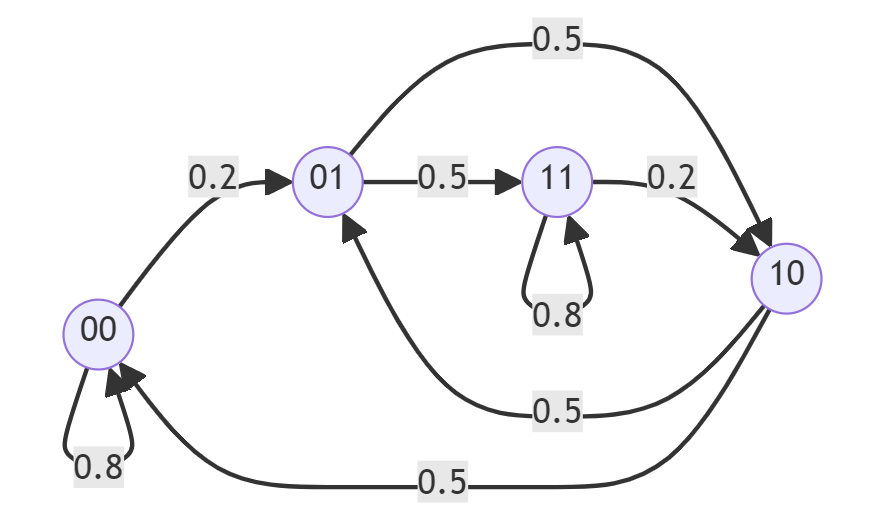
\includegraphics[width=0.5\textwidth]{./img/mermaid1.png}
\end{figure}

\textbf{
Calcula las probabilidades de los estados en estado estacionario y la entropía de la fuente.
}

\vspace{1cm}

\textbf{
10. Sea una fuente de Markov de primer orden sobre el alfabeto $\mathcal{S}=\left\{a,b,c\right\}$ definida por el siguiente diagrama de estados:
}

\begin{figure}[htbp!]
    \centering
    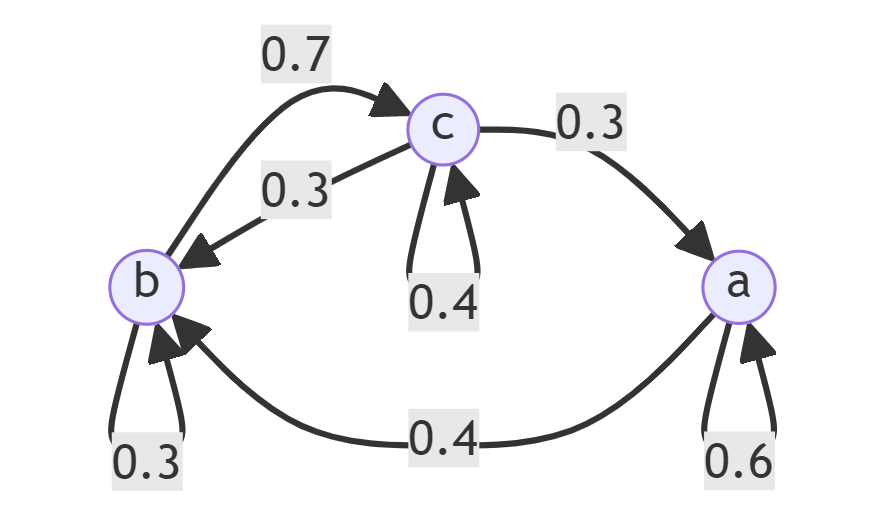
\includegraphics[width=0.5\textwidth]{./img/mermaid2.png}
\end{figure}

\textbf{Calcula:}

\begin{itemize}
    \item\textbf{La probabilidad de cata estado en régimen estacionario.}
    \item\textbf{La entropía de la fuente.}
    \item\textbf{La fuente afín.}
    \item\textbf{La entropía de La fuente afín.}
\end{itemize}


\end{document}